% CabinGuard-ADI architecture, colour version of Fig. 1 of the paper for the README.
% Same blocks, signals and arrows as the paper's TikZ figure; only the styling differs.
% Build: pdflatex architecture.tex && pdftoppm -png -r 300 -singlefile architecture.pdf architecture
\documentclass[border=10pt]{standalone}
\usepackage[scaled=0.95]{helvet}
\renewcommand{\familydefault}{\sfdefault}
\usepackage{amsmath}
\usepackage{tikz}
\usetikzlibrary{arrows.meta,positioning,calc,fit,backgrounds,shadows}

% stage colours (colour-blind safe categorical slots, pale fills)
\definecolor{cSense}{HTML}{2a78d6}
\definecolor{cFeat}{HTML}{6250d6}
\definecolor{cEvid}{HTML}{1baf7a}
\definecolor{cDec}{HTML}{eb6834}
\definecolor{cVeh}{HTML}{0b0b0b}
\definecolor{cEm}{HTML}{e34948}
\definecolor{ink}{HTML}{1f1f1d}
\definecolor{ink2}{HTML}{52514e}

\begin{document}
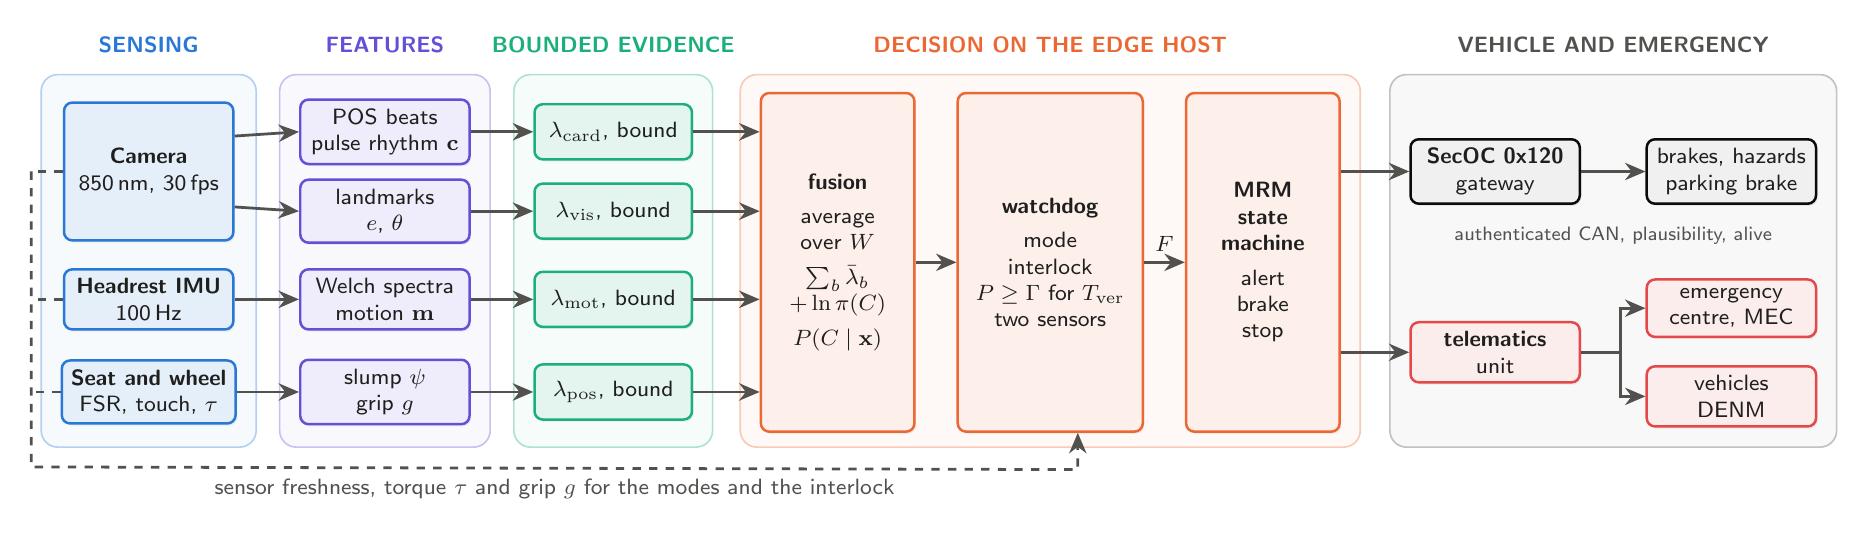
\begin{tikzpicture}[x=1.0cm, y=1.12cm,
  font=\footnotesize, >={Stealth[length=2.6mm, width=2.2mm]},
  base/.style={rounded corners=3pt, line width=0.9pt, align=center, text=ink,
               minimum height=0.7cm, drop shadow={opacity=0.12, shadow xshift=0.6pt, shadow yshift=-0.8pt}},
  sen/.style={base, draw=cSense, fill=cSense!12, minimum width=2.15cm},
  feat/.style={base, draw=cFeat, fill=cFeat!10, minimum width=2.15cm},
  evid/.style={base, draw=cEvid, fill=cEvid!12, minimum width=2.0cm},
  dec/.style={base, draw=cDec, fill=cDec!10},
  veh/.style={base, draw=cVeh, fill=cVeh!6, minimum width=2.15cm},
  em/.style={base, draw=cEm, fill=cEm!10, minimum width=2.15cm},
  arr/.style={->, line width=1.0pt, draw=ink2},
  stage/.style={font=\footnotesize\bfseries, anchor=south},
  ]
  % ---------------------------------------------------------------- blocks (as in the paper)
  \node[sen, minimum height=1.75cm] (cam) at (0,3.0) {\textbf{Camera}\\850\,nm, 30\,fps};
  \node[sen] (imu) at (0,1.55) {\textbf{Headrest IMU}\\100\,Hz};
  \node[sen] (seat) at (0,0.5) {\textbf{Seat and wheel}\\FSR, touch, $\tau$};
  \node[feat] (fc) at (3.0,3.45) {POS beats\\pulse rhythm $\mathbf{c}$};
  \node[feat] (fv) at (3.0,2.55) {landmarks\\$e$, $\theta$};
  \node[feat] (fm) at (3.0,1.55) {Welch spectra\\motion $\mathbf{m}$};
  \node[feat] (fp) at (3.0,0.5) {slump $\psi$\\grip $g$};
  \node[evid] (bc) at (5.9,3.45) {$\lambda_{\mathrm{card}}$, bound};
  \node[evid] (bv) at (5.9,2.55) {$\lambda_{\mathrm{vis}}$, bound};
  \node[evid] (bm) at (5.9,1.55) {$\lambda_{\mathrm{mot}}$, bound};
  \node[evid] (bp) at (5.9,0.5) {$\lambda_{\mathrm{pos}}$, bound};
  \node[dec, minimum height=4.3cm, minimum width=1.95cm] (fu) at (8.75,1.97)
       {\textbf{fusion}\\[3pt]average\\over $W$\\[3pt]$\sum_b\bar\lambda_b$\\$+\ln\pi(C)$\\[3pt]$P(C\mid\mathbf{x})$};
  \node[dec, minimum height=4.3cm, minimum width=2.35cm] (wd) at (11.45,1.97)
       {\textbf{watchdog}\\[3pt]mode\\interlock\\$P\ge\Gamma$ for $T_{\mathrm{ver}}$\\two sensors};
  \node[dec, minimum height=4.3cm, minimum width=1.95cm] (sm) at (14.15,1.97)
       {\textbf{MRM}\\\textbf{state}\\\textbf{machine}\\[3pt]alert\\brake\\stop};
  \node[veh] (gw) at (17.1,3.0) {\textbf{SecOC 0x120}\\gateway};
  \node[veh] (act) at (20.1,3.0) {brakes, hazards\\parking brake};
  \node[em] (tel) at (17.1,0.95) {\textbf{telematics}\\unit};
  \node[em] (psap) at (20.1,1.45) {emergency\\centre, MEC};
  \node[em] (v2x) at (20.1,0.45) {vehicles\\DENM};

  % ---------------------------------------------------------------- arrows (as in the paper)
  \draw[arr] ([yshift=0.45cm]cam.east) -- (fc.west);
  \draw[arr] ([yshift=-0.45cm]cam.east) -- (fv.west);
  \draw[arr] (imu) -- (fm);
  \draw[arr] (seat) -- (fp);
  \draw[arr] (fc) -- (bc); \draw[arr] (fv) -- (bv); \draw[arr] (fm) -- (bm); \draw[arr] (fp) -- (bp);
  \draw[arr] (bc.east) -- (bc.east -| fu.west);
  \draw[arr] (bv.east) -- (bv.east -| fu.west);
  \draw[arr] (bm.east) -- (bm.east -| fu.west);
  \draw[arr] (bp.east) -- (bp.east -| fu.west);
  \draw[arr] (fu) -- (wd);
  \draw[arr] (wd) -- node[above, text=ink]{$F$} (sm);
  \draw[arr] (sm.east |- gw.west) -- (gw.west);
  \draw[arr] (sm.east |- tel.west) -- (tel.west);
  \draw[arr] (gw) -- (act);
  \draw[arr] (tel.east) -- ++(0.5,0) |- (psap.west);
  \draw[arr] (tel.east) -- ++(0.5,0) |- (v2x.west);
  \draw[line width=1.0pt, dashed, draw=ink2] (cam.west) -- ++(-0.4,0) coordinate (h1);
  \draw[line width=1.0pt, dashed, draw=ink2] (imu.west) -- ++(-0.4,0);
  \draw[line width=1.0pt, dashed, draw=ink2] (seat.west) -- ++(-0.4,0);
  \draw[arr, dashed] (h1) -- ++(0,-3.35) -- node[pos=0.5, below, text=ink2]{sensor freshness, torque $\tau$ and grip $g$ for the modes and the interlock}
        ([xshift=0.35cm]wd.south |- 0,-0.38) -- ([xshift=0.35cm]wd.south);

  % ---------------------------------------------------------------- stage headings and bands
  \coordinate (bandtop) at (0cm,4.45cm);
  \coordinate (bandbot) at (0cm,0cm);
  \coordinate (heady) at (0cm,4.75cm);
  \coordinate (vmid) at ($(gw.north)!0.5!(act.north)$);
  \begin{scope}[on background layer]
    % every band spans the same height, so the stage headings line up
    \foreach \a/\b/\c in {cam/seat/cSense, fc/fp/cFeat, bc/bp/cEvid, fu/sm/cDec, gw/v2x/ink2} {
      \node[fit=(\a)(\b)(\a.north |- bandtop)(\b.south |- bandbot), inner xsep=7pt, inner ysep=4pt,
             rounded corners=6pt, fill=\c!4, draw=\c!35, line width=0.6pt] {};
    }
  \end{scope}
  \node[stage, text=cSense] at (cam.north |- heady) {SENSING};
  \node[stage, text=cFeat] at (fc.north |- heady) {FEATURES};
  \node[stage, text=cEvid] at (bc.north |- heady) {BOUNDED EVIDENCE};
  \node[stage, text=cDec] at (wd.north |- heady) {DECISION ON THE EDGE HOST};
  \node[stage, text=ink2] at (vmid |- heady) {VEHICLE AND EMERGENCY};
  \node[font=\scriptsize, text=ink2, align=center] at ($(gw.south)!0.5!(act.south)+(0,-0.35)$) {authenticated CAN, plausibility, alive};
\end{tikzpicture}
\end{document}
